\startchapter{Results}
\label{chapter:eval}

This chapter presents the results of the comparison between distance-based spatial interpolation methods (IDW, Kriging) and physics-based parameter estimation methods (4D-Var, GLM, IES) for the reconstruction of PHC plume distributions from sparse sensor measurements. The evaluation proceeds in two stages. Section~\ref{sec:synth_results} presents results on the synthetic dataset, beginning with a base case that establishes the reference performance of each method and the comparison format used throughout. Then the performance under the controlled variations described in Section~\ref{sec:synth_var}: measurement noise, sensor count, measurement frequency, soil parameter noise, and sensor dropout is examined. These variations are designed to test each method's robustness under conditions representative of real-world deployment, allowing the relative strengths and failure modes of each approach to be identified rather than relying on a single point of comparison. Computational cost is also reported for each method, since practical deployment must weigh reconstruction accuracy against runtime. Section~\ref{sec:real_world_results} then validates these findings against the real-world dataset collected from an active remediation site, assessing whether the trends observed under synthetic conditions persist when applied to field data with its associated irregularities and reduced sample size.

Together, these results address the central problem motivating this thesis: identifying a suitable method for reconstructing PHC plume distributions from the sparse sensor networks in active biostimulation remediation sites. As shown below, the physics-based parameter estimation methods consistently outperform the distance-based methods across nearly all conditions tested, with IES achieving the best overall accuracy at the cost of substantially higher computational expense. 

\section{Synthetic Data}
\label{sec:synth_results}
The synthetic results are organized around the data variations described in Chapter~\ref{chapter:Exp}. Each method is compared under each condition, beginning with the base case to establish a reference point and the comparison format used throughout.

\subsection{Base Case}

The base case uses zero measurement error, zero soil parameter noise, two-month measurement windows with 12-hour sampling frequency, and no sensor dropout.

\begin{figure}[!h]
    \centering
    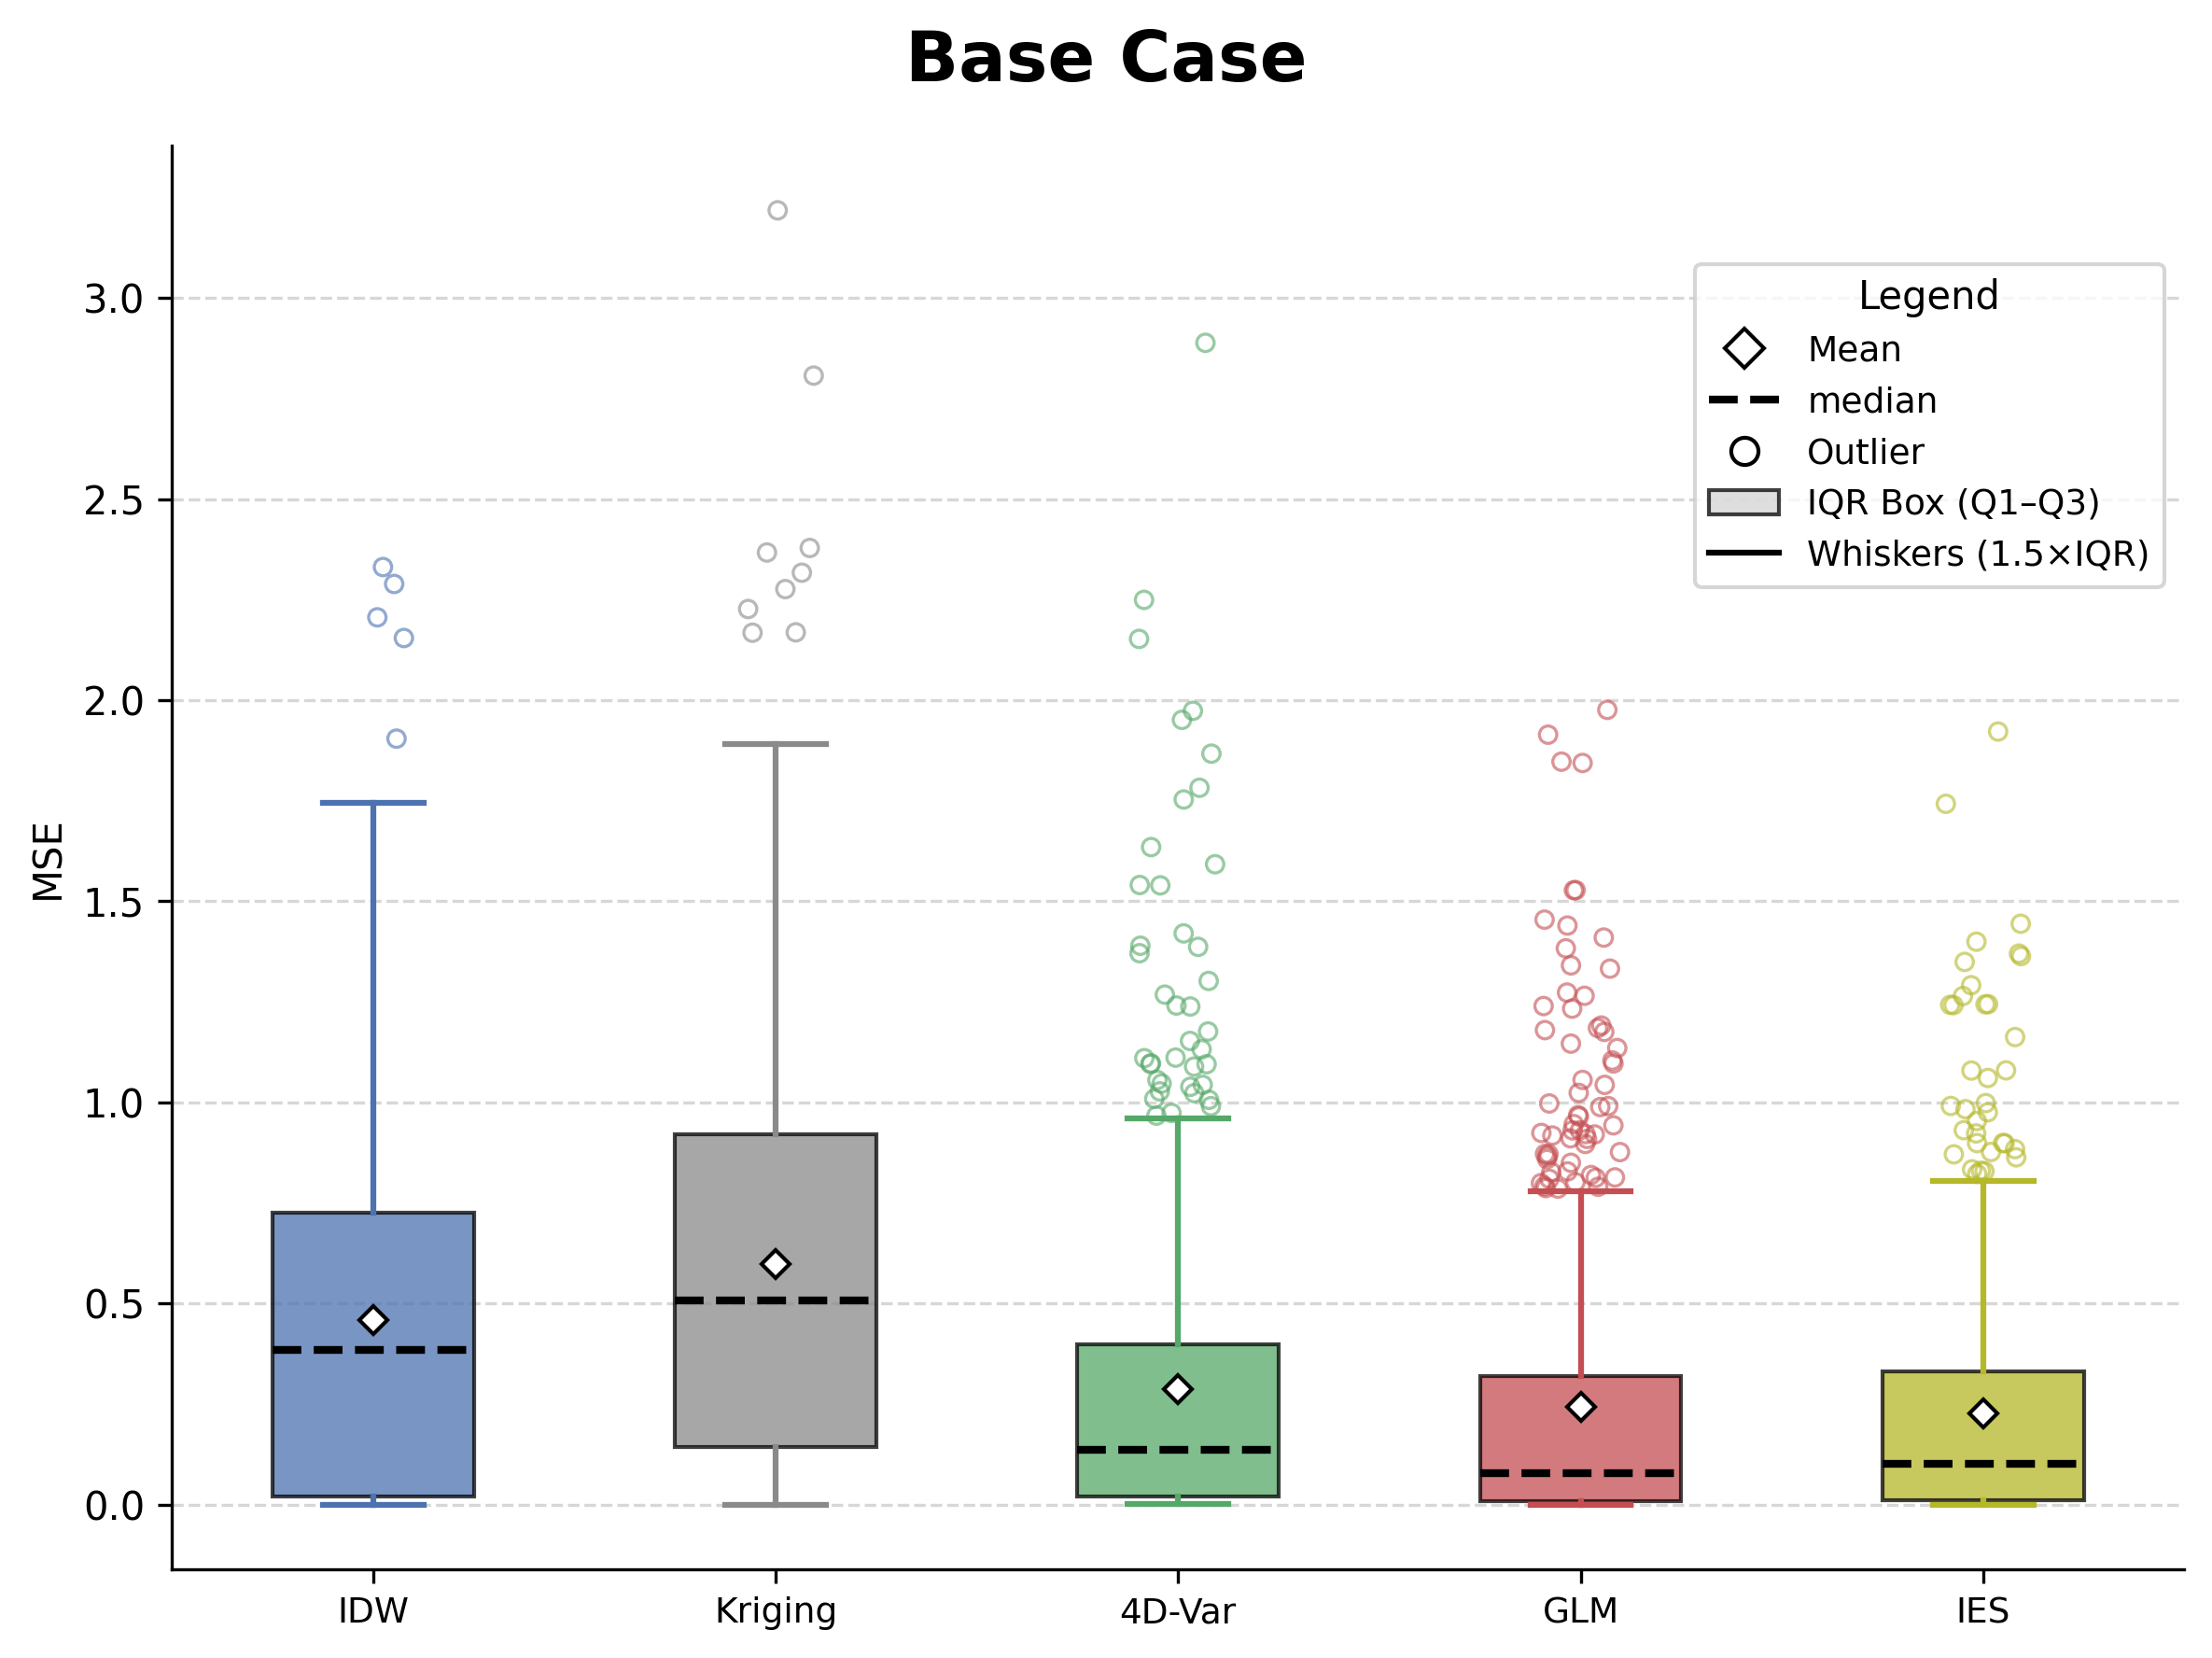
\includegraphics[width=5in]{figures/base_case.png}
    \caption{Boxplot results for all $\valsize$ synthetic samples evaluated by each method.}
    \label{fig:res_baseCase}
\end{figure}

For clarity, the components of the boxplot are described briefly here: the white diamond marks the mean, the dashed line marks the median, the box spans the interquartile range (25th to 75th percentile), and the whiskers extend to the furthest data point that lies within 1.5 times the interquartile range beyond the box edges. Points beyond the whiskers are plotted individually as outliers. This format is used consistently for all boxplots throughout the remainder of this chapter.

% 5 numbers to change here!!!
The base case results clearly foreshadow the trends that persist throughout the remaining variations. The physics-based parameter estimation methods substantially outperform the distance-based methods in reconstructing the spatial distribution of the PHC plume. The most striking difference is not in the mean MSE but in the median. The parameter estimation methods place significantly more samples in the low-error regime, with median MSE values of 0.1018 for IES, 0.0778 for GLM, and 0.1367 for 4D-Var, compared to 0.3835 for IDW and 0.5066 for Kriging. The parameter estimation methods do still produce some high-error outliers, which inflates their mean values. Their narrower interquartile ranges reinforce the conclusion that the physics-informed approach more consistently yield lower errors. Four samples from each method are shown in Figure~\ref{fig:res_combined}, one for each of the source locations described in Section~\ref{sec:synth_soil_params}.

Among the parameter estimation methods, 4D-Var performs worst, followed by GLM, with IES performing best by a small margin over GLM. This ranking correlates strongly with the number of forward model runs each method completes. IES, with its large ensemble, executes substantially more model evaluations than the other two. Likewise, GLM runs more forward models than 4D-Var due to its finite-difference gradient approximation. The model run counts for each method are shown in Figure~\ref{fig:res_nModelRuns}. These results also roughly correspond to the runtimes of the models which can be seen in Figure~\ref{fig:res_nModelTimes}. These individual results were selected to showcase the strengths and weaknesses of each model. Inverse Distance Weighting is unable to capture the concentrations towards the boundary conditions due to the sensor locations and its pure distance-based interpolation. Similarly, Kriging does not capture these boundary condition dynamics. Because the semi-variance is limited to 3 points the calibrated linear model cannot accurately represent the data. This effect is due in part to the automatic  calibration of the linear weights, however in the best case it would likely not outperform IDW. The parameter estimation methods utilize the physical constraints to predict the boundary condition dynamics in the top and bottom source locations, but are prone to overestimating the boundary conditions visible clearly in the no source example. 

\begin{figure}[H]
    \centering
    \includegraphics[width=6.5in]{figures/combined.png}
    \caption{Sample results from synthetic data samples. Columns correspond to methods: IDW, Kriging, 4D-Var, GLM and IES. Rows correspond to top, bottom, both and no source locations. Orange lines depict the spatial truth. Blue dashed lines depict the estimates of IDW, Kriging, 4D-Var, GLM. IES depicts its estimate as a heatmap of ensemble members.}
    \label{fig:res_combined}
\end{figure}

\begin{figure}[H]
    \centering
    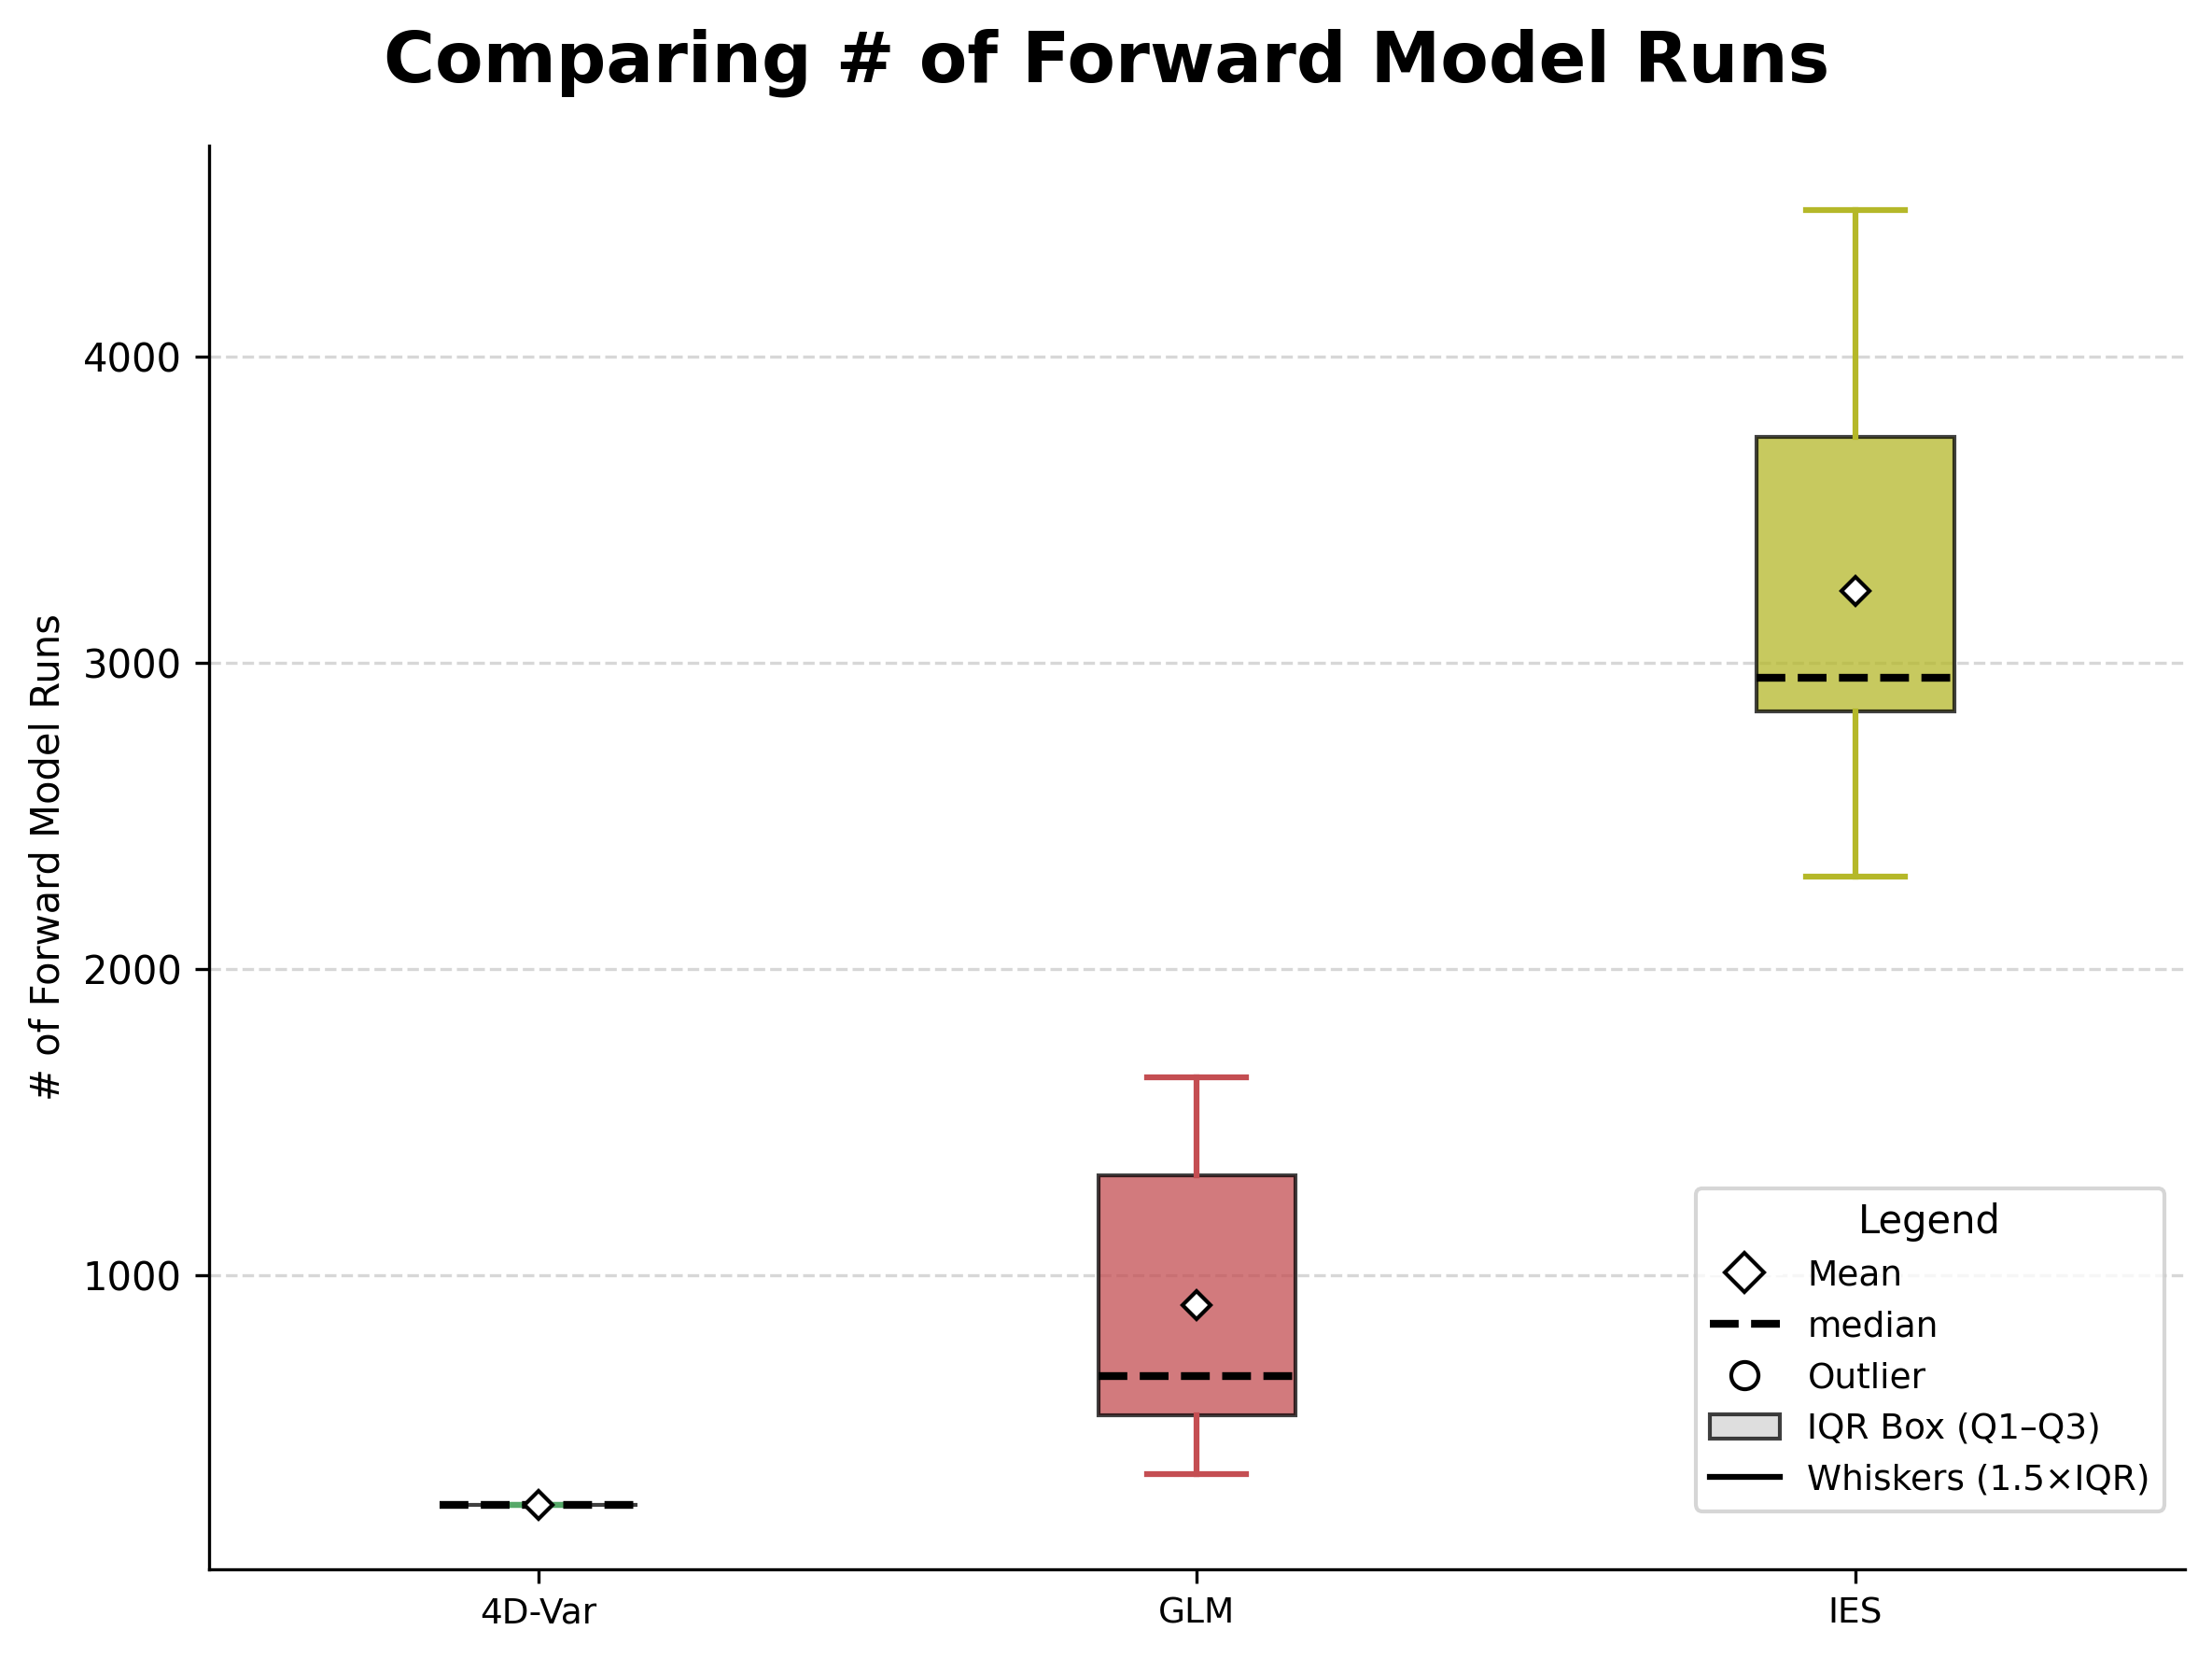
\includegraphics[width=5in]{figures/nModel_runs.png}
    \caption{Number of forward model runs completed by each parameter estimation method.}
    \label{fig:res_nModelRuns}
\end{figure}



\begin{figure}[H]
    \centering
    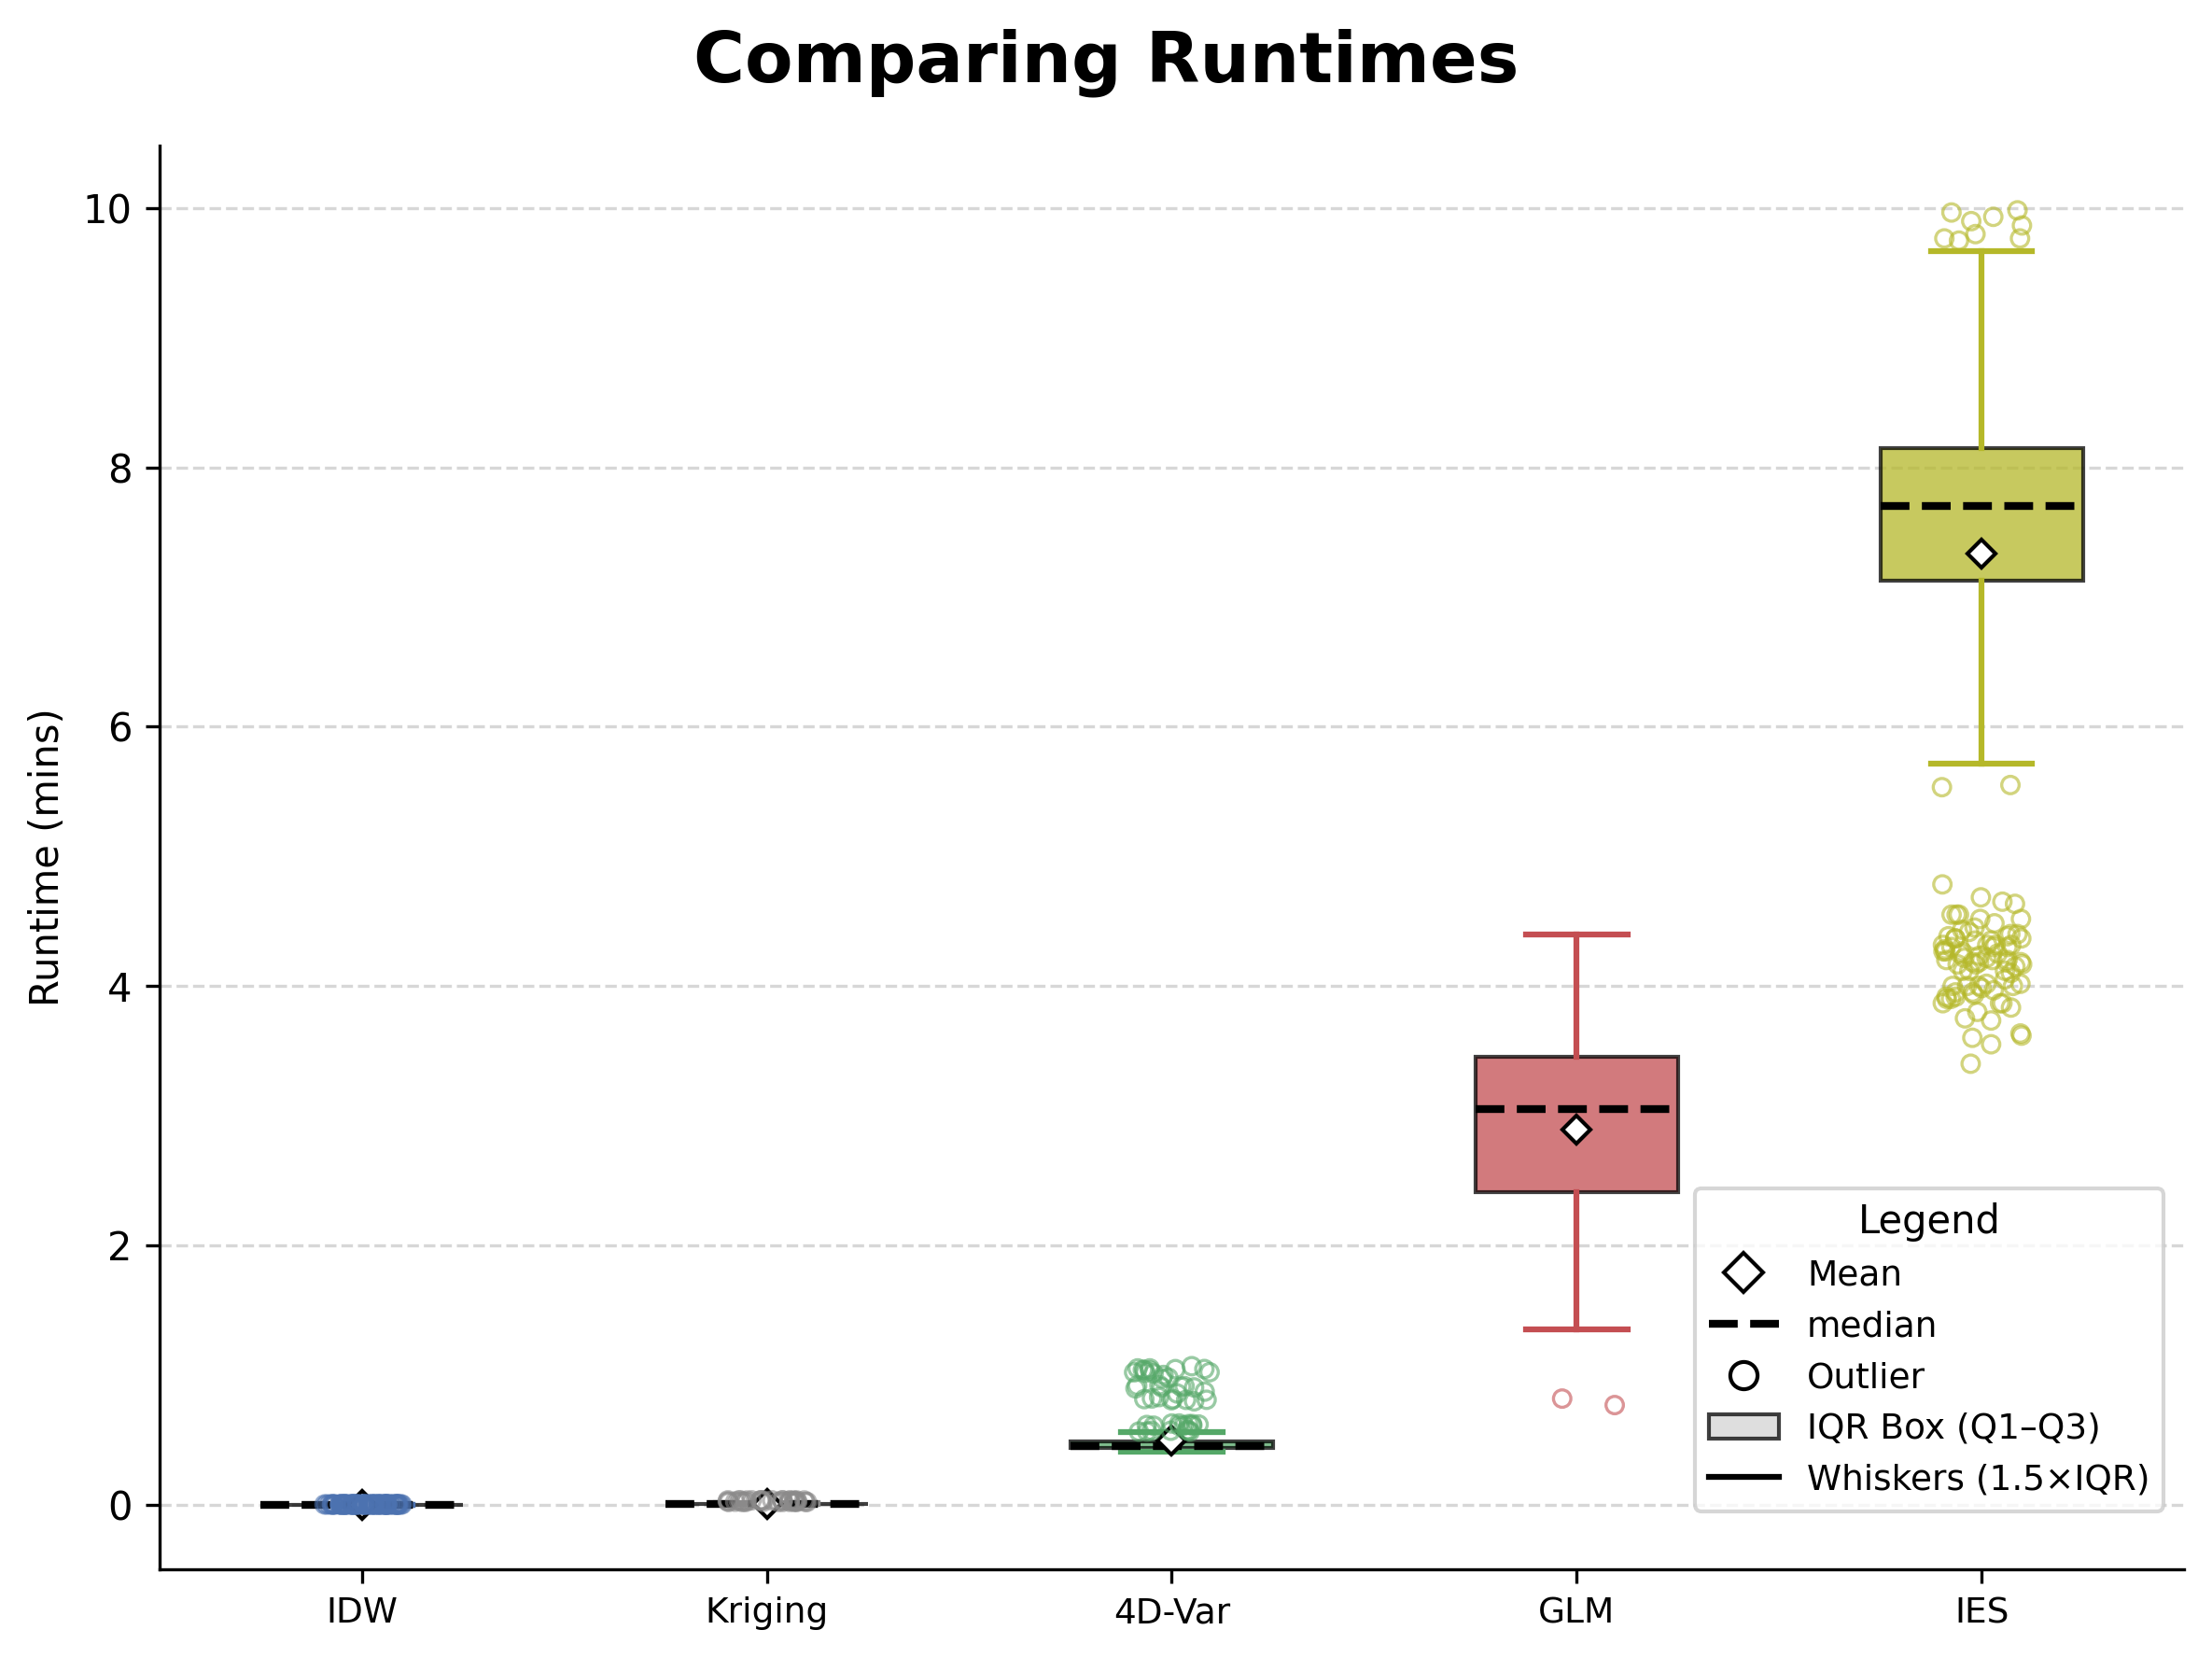
\includegraphics[width=5in]{figures/nModel_times.png}
    \caption{Runtime of each parameter estimation method in minutes measured with serial execution on a single CPU core}
    \label{fig:res_nModelTimes}
\end{figure}

Executed on a single-core of a CPU, the distance-based methods operate in well under one second per sample: IDW at $1.27 \times 10^{-5}$~min and Kriging at $4.9 \times 10^{-3}$~min. Among the parameter estimation methods, 4D-Var is the fastest at 0.49~min, benefiting from the adjoint model which minimizes the number of forward evaluations (Figure~\ref{fig:res_nModelRuns}). GLM takes approximately $2.89$~min, roughly 6 times longer than 4D-Var. This reflects the cost of its finite-difference gradient estimation, which requires multiple forward runs per iteration. IES is the most expensive at $7.3$~min, approximately 15 times the cost of 4D-Var and 2.5$\times$ that of GLM, consistent with its large ensemble of parallel simulations. The performance advantage of IES over GLM in most conditions must therefore be weighed against this substantial additional cost.


\begin{figure}[H]
    \centering
    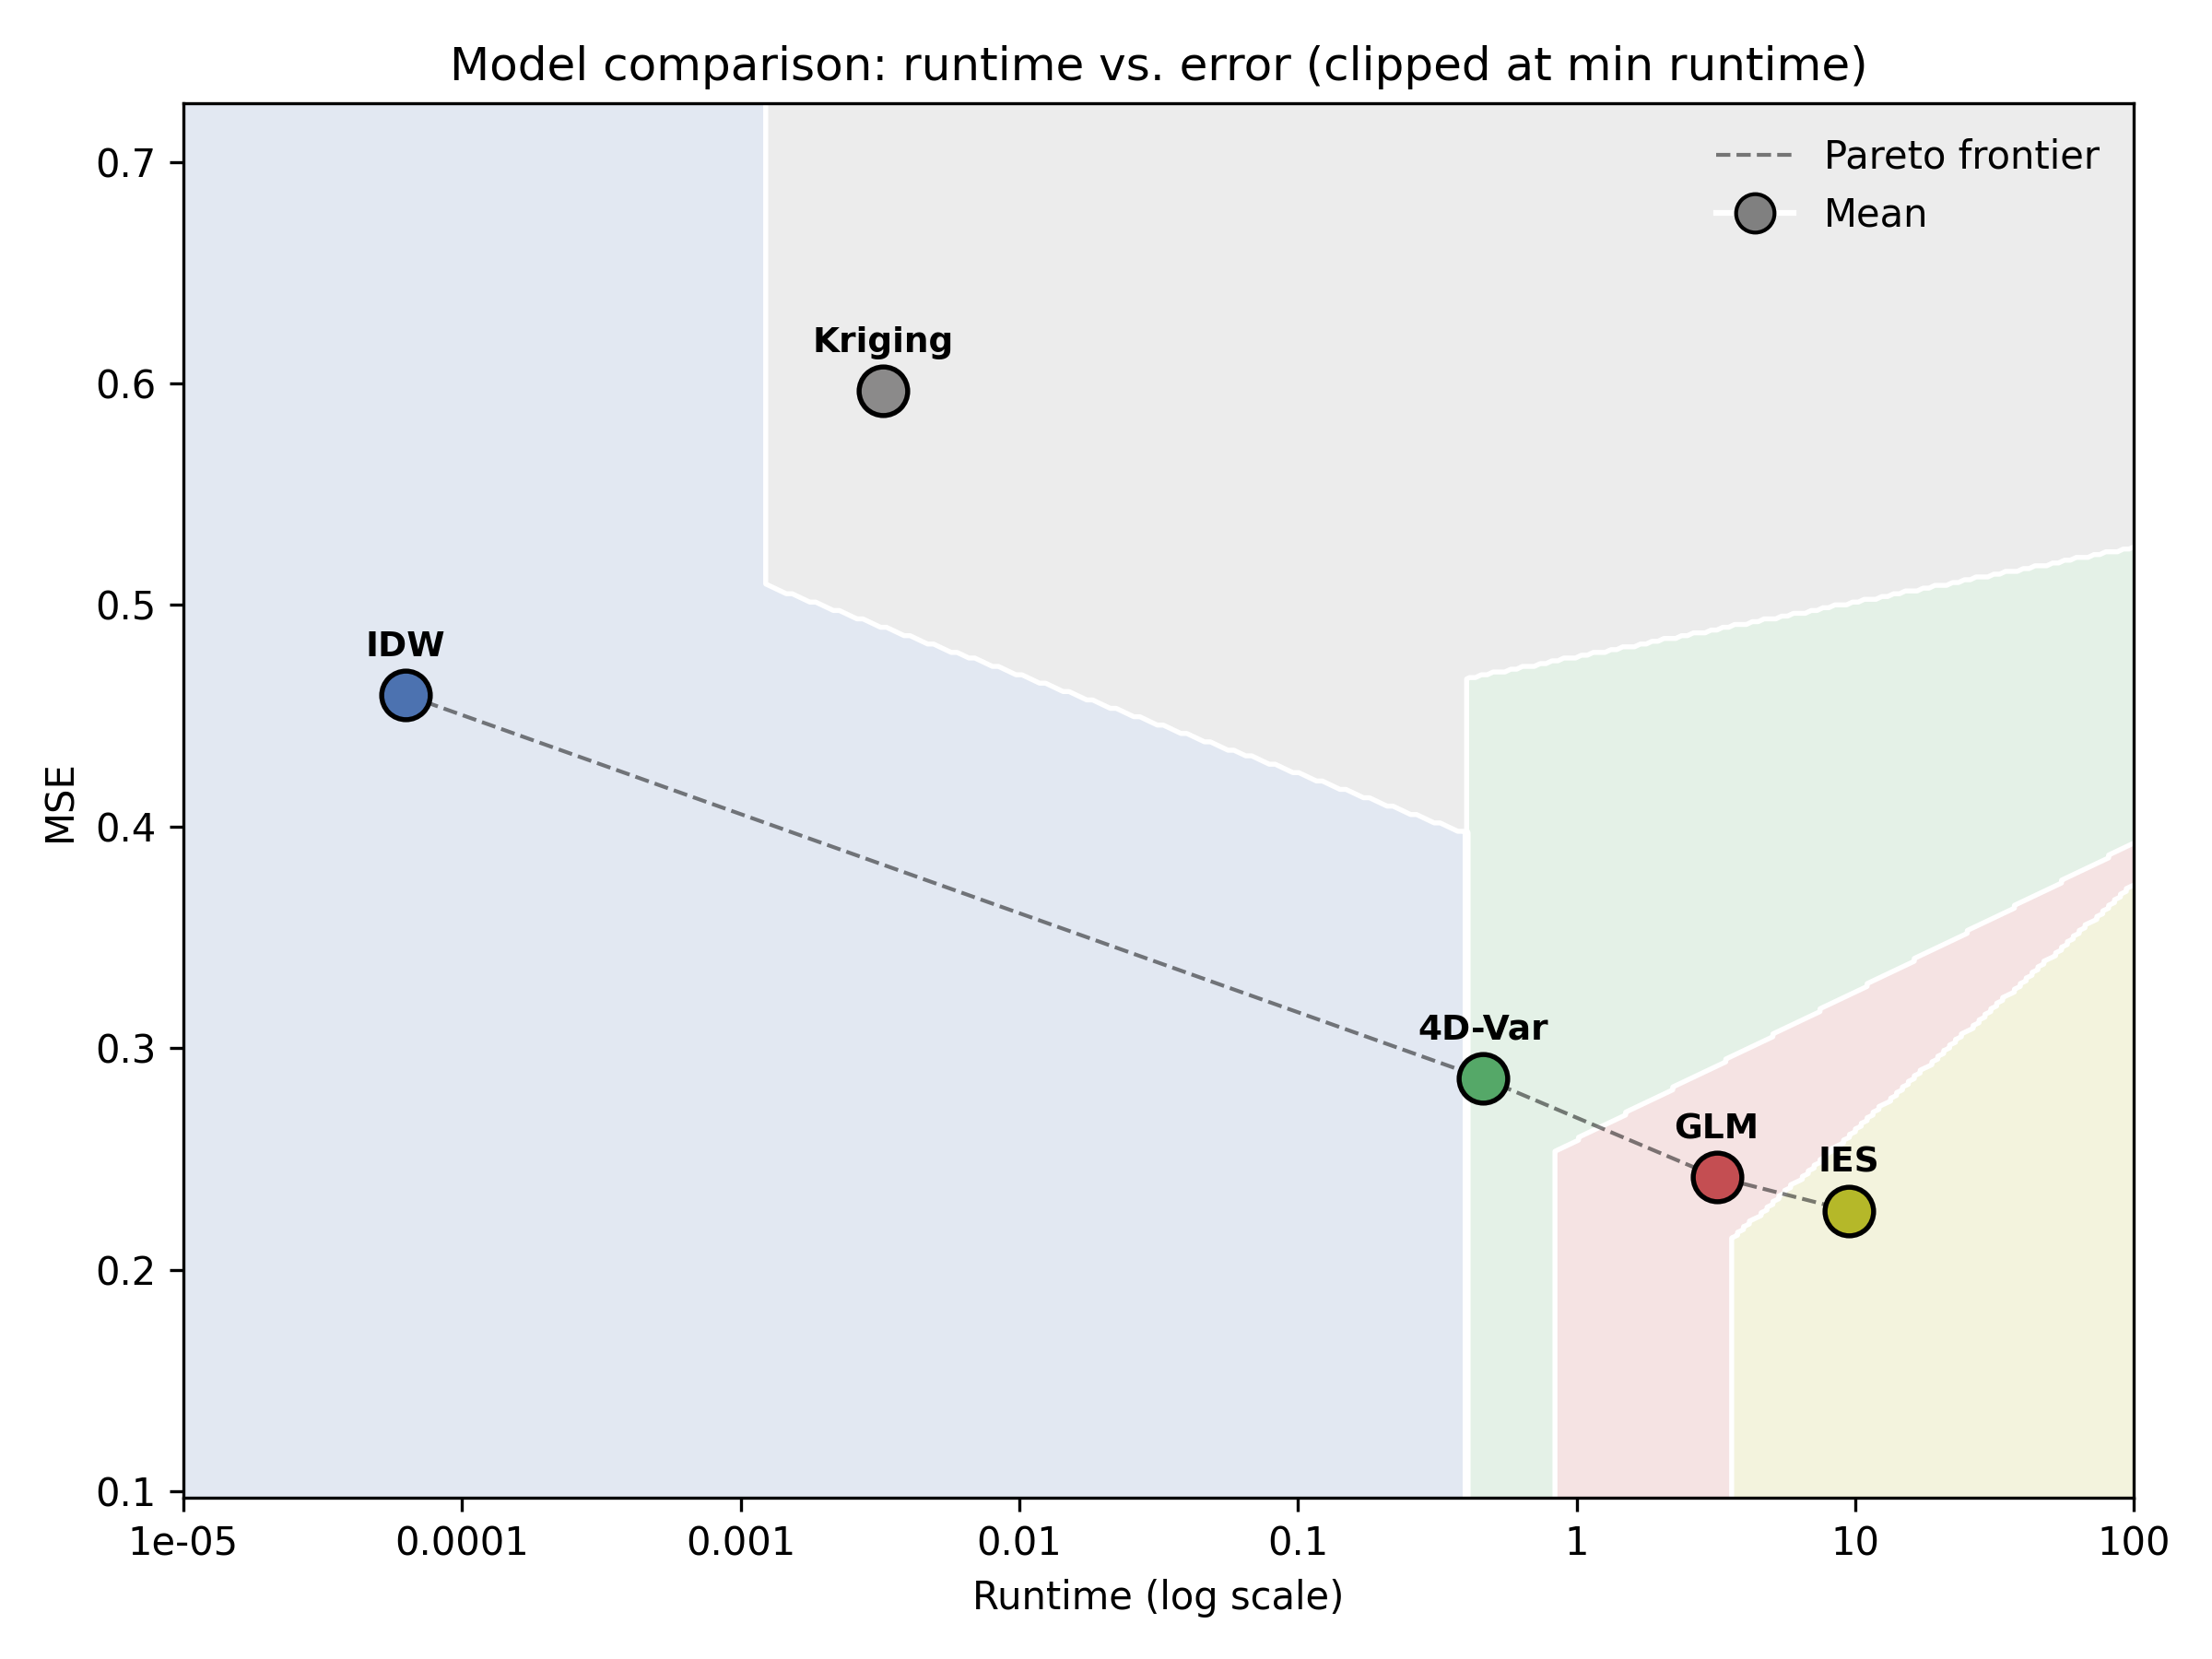
\includegraphics[width=6in]{figures/error_v_runtime.png}
    \caption{Model runtime plotted against mean squared error (MSE) for each parameter estimation method. The solid marker gives the mean runtime and mean MSE across all runs of a given method. The surrounding area is a voronoi diagram, however the areas are clipped at the shortest recorded runtime of the respective method.}
    \label{fig:runtime_v_error}
\end{figure}

Figure~\ref{fig:runtime_v_error} plots runtime directly against mean MSE for each method, making clear which methods are useful at which timescales. Below roughly 0.5~min, IDW is the best choice, achieving a lower mean MSE than Kriging while running two orders of magnitude faster ($1.27\times10^{-5}$~min vs.\ $4.9\times10^{-3}$~min) on average, which means Kriging is never the preferred option regardless of the available time budget. This regime, spanning from $1.27\times10^{-5}$ to roughly 0.3~min, is well suited to real-time and edge-compute settings where decisions must be immediately made from observations. With more than 0.3~min of compute, 4D-Var becomes the superior method, improving substantially on IDW's average MSE. At this timescale, edge-compute is still plausible, though the runtime is more realistic for a post-processing setting. GLM and IES occupy the slower end of the timescale and are firmly restricted to post-processing use, but both further reduce mean MSE relative to 4D-Var. Comparing the two, IES improves on both the mean and standard deviation of MSE relative to GLM. Therefor, GLM is the preferable choice when post-processing compute is constrained by model size, while IES is preferable when accuracy is more important than compute


Before proceeding to the variations, it is worth confirming that the $\valsize$-sample dataset is sufficiently large to support reliable conclusions. Figure~\ref{fig:res_sePlot} shows the running mean and 95\% confidence interval (standard error) for each method as a function of sample count.

\begin{figure}[!h]
    \centering
    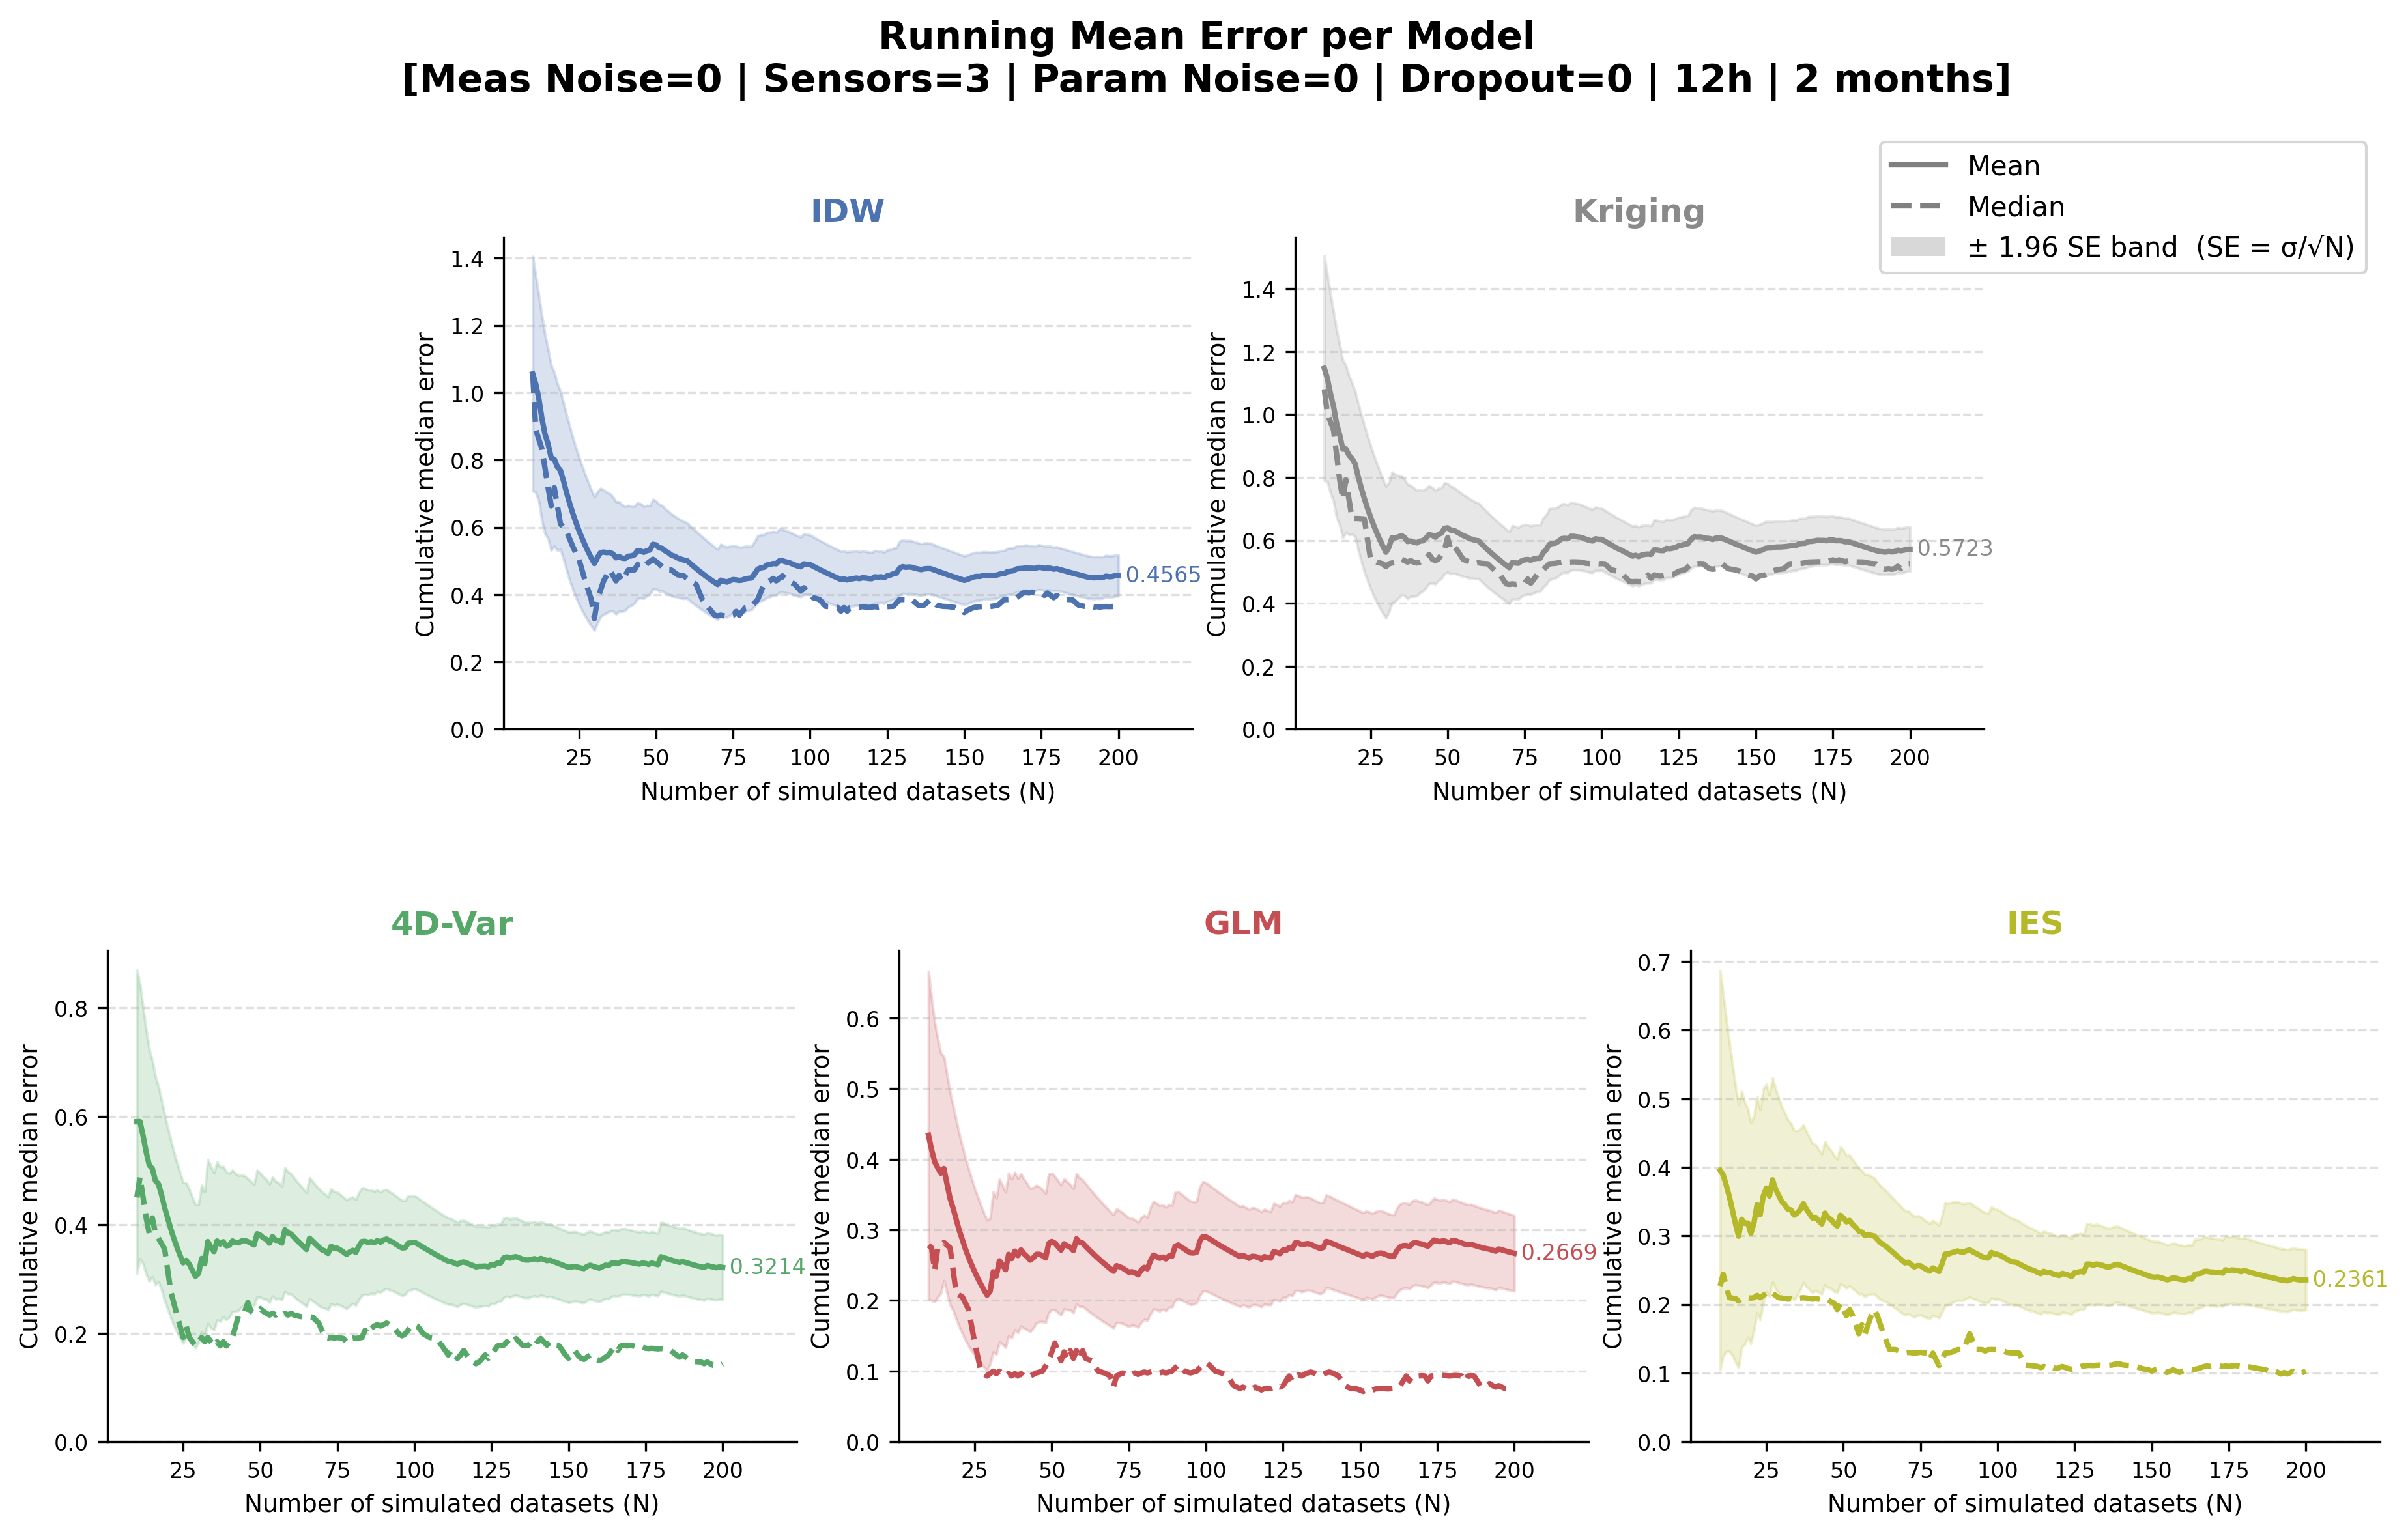
\includegraphics[width=6in]{figures/running_mean_single_testcase.png}
    \caption{Running mean and 95\% confidence interval (standard error) for each method, illustrating the representativeness of the $\valsize$-sample results.}
    \label{fig:res_sePlot}
\end{figure}

The confidence intervals for the distance-based methods demonstrate that the gap between the parameter estimation group and the distance-methods is unambiguous. Among the parameter estimation methods, the confidence interval of 4D-Var solidifies that 4D-Var does not perform as well as the other parameter estimation methods. However, the difference between GLM and IES is less certain due to their overlapping confidence intervals. The complete numerical results for all conditions are summarized in Table~\ref{tab:sim_results}.


% Auto-generated LaTeX table
\begin{table}[htbp]
  \centering
  \caption{Model performance under varying conditions (MSE)}
  \label{tab:sim_results}
  \begin{tabular}{lrrrrr}
  \toprule
  Condition & IDW & Kriging & 4D-Var & GLM & IES \\
  \midrule
  \multicolumn{6}{l}{\textit{Mean}} \\
  \hline
  Base Case & 0.4595 & 0.5969 & 0.2865 & 0.2419 & \textbf{0.2266} \\
  0.001\% Meas Noise & 0.4589 & 0.5694 & 0.2881 & 0.2447 & \textbf{0.2327} \\
  0.01\% Meas Noise & 0.4594 & 0.5952 & 0.2799 & 0.2536 & \textbf{0.2317} \\
  4 Sensors & 0.1983 & 0.6382 & 0.1567 & 0.1525 & \textbf{0.1195} \\
  1 Sensor & 0.7582 &  & 0.7321 & \textbf{0.7196} & 0.7499 \\
  2 Sensors & 0.4743 & 1.094 & 0.2953 & \textbf{0.2685} & 0.2786 \\
  4 Hour Measurements & 0.4566 & 0.5634 & 0.2811 & 0.259 & \textbf{0.227} \\
  0.01 Param Noise & 0.559 & 0.7078 & 0.4617 & 0.4849 & \textbf{0.433} \\
  0.1 Param Noise & \textbf{1.353} & 1.413 & 1.624 & 1.569 & 1.597 \\
  10\% Sens Dropout & 0.4342 & 0.5827 & 0.2577 & 0.199 & \textbf{0.1915} \\
  50\% Sens Dropout & 0.4276 & 0.5498 & 0.3118 & 0.2131 & \textbf{0.1971} \\
  50\% Sens Blackout & 0.4178 & 0.6277 & 0.2476 & 0.187 & \textbf{0.1838} \\
  \midrule
  \multicolumn{6}{l}{\textit{Median}} \\
  \hline
  Base Case & 0.3835 & 0.5066 & 0.1367 & \textbf{0.0778} & 0.1018 \\
  0.001\% Meas Noise & 0.3851 & 0.5022 & 0.1491 & \textbf{0.07379} & 0.1085 \\
  0.01\% Meas Noise & 0.3825 & 0.5691 & 0.1354 & \textbf{0.0947} & 0.1025 \\
  4 Sensors & 0.08858 & 0.4702 & 0.06511 & 0.03908 & \textbf{0.02754} \\
  1 Sensor & 0.6943 &  & 0.5467 & \textbf{0.5407} & 0.5949 \\
  2 Sensors & 0.4121 & 0.8268 & 0.1699 & \textbf{0.09641} & 0.1701 \\
  4 Hour Measurements & 0.3802 & 0.5027 & 0.1386 & \textbf{0.08853} & 0.1015 \\
  0.01 Param Noise & 0.4404 & 0.5994 & 0.2698 & 0.2545 & \textbf{0.2261} \\
  0.1 Param Noise & \textbf{1.104} & 1.21 & 1.366 & 1.275 & 1.316 \\
  10\% Sens Dropout & 0.3595 & 0.4914 & 0.1237 & \textbf{0.03372} & 0.1006 \\
  50\% Sens Dropout & 0.3427 & 0.4852 & 0.1611 & \textbf{0.05765} & 0.09836 \\
  50\% Sens Blackout & 0.3382 & 0.5615 & 0.1119 & \textbf{0.05316} & 0.1004 \\
  \midrule
  \multicolumn{6}{l}{\textit{Standard Deviation}} \\
  \hline
  Base Case & 0.4339 & 0.5217 & 0.3854 & 0.3503 & \textbf{0.2997} \\
  0.001\% Meas Noise & 0.4338 & 0.5061 & 0.3832 & 0.3589 & \textbf{0.3057} \\
  0.01\% Meas Noise & 0.4338 & 0.4946 & 0.3616 & 0.3548 & \textbf{0.3027} \\
  4 Sensors & 0.2404 & 0.6816 & 0.241 & 0.2184 & \textbf{0.1994} \\
  1 Sensor & \textbf{0.6523} &  & 0.7454 & 0.7111 & 0.6815 \\
  2 Sensors & 0.4402 & 1.06 & 0.3526 & 0.3791 & \textbf{0.3232} \\
  4 Hour Measurements & 0.433 & 0.4906 & 0.3649 & 0.3665 & \textbf{0.2986} \\
  0.01 Param Noise & 0.5693 & 0.6589 & 0.5634 & 0.5842 & \textbf{0.5611} \\
  0.1 Param Noise & 1.297 & \textbf{1.287} & 1.535 & 1.499 & 1.551 \\
  10\% Sens Dropout & 0.3925 & 0.5203 & 0.3433 & 0.2944 & \textbf{0.2153} \\
  50\% Sens Dropout & 0.4058 & 0.4983 & 0.4541 & 0.327 & \textbf{0.2429} \\
  50\% Sens Blackout & 0.3948 & 0.541 & 0.3438 & 0.2979 & \textbf{0.2134} \\
  \bottomrule
  \end{tabular}
\end{table}


% 5 numbers to change here!!!
\subsection{Measurement Noise}
\label{sec:res_measNoise}
As shown in Table~\ref{tab:sim_results}, measurement noise has minimal effect on any of the methods. The distance-based methods are largely insensitive to temporal perturbations by design, so their stability is unsurprising. Among the parameter estimation methods, 4D-Var's mean MSE actually improves from 0.2865 at the base case to 0.2799 at 0.01\% noise, a reduction of roughly 2.4\%. A plausible explanation is that the added noise acts as a form of regularisation, discouraging over-fitting to the temporal measurements and preventing the optimiser from converging to extreme parameter distributions; however it is likely that the change is too small to be conclusive. GLM and IES, the best overall performers, show a marginal increase in mean MSE from 0.2419 to 0.2536 and 0.2266 to 0.2317 at the highest noise level, but this change is small enough to be inconclusive. Median MSE and standard deviation follow similar patterns, with the standard deviation of the parameter estimation methods decreasing slightly under higher noise, consistent with the regularisation hypothesis.

\subsection{Number of Sensors}
 
The sensor count results reveal several notable crossover points. Kriging remains ineffective regardless of sensor count: even with four sensors, the empirical variogram contains only 6 points, which is insufficient for reliable fitting.
% 8 numbers to change here!!!
With four sensors, IDW achieves a mean MSE of 0.1983, comparable to 4D-Var at 0.1567 and only 1.6 times larger than the best-performing method (IES at 0.1195). The additional sensor near the surface gives IDW better visibility of the boundary conditions which benefits IDW's averaging approach disproportionately in this setting. With a single sensor, the parameter estimation methods degrade substantially, with 4D-Var (0.7321) and IES (0.7499) perform comparably to IDW (0.7582), and only GLM (0.7196) marginally outperforms them. With only one measurement time series, the parameter estimation methods lack the spatial context needed to constrain the simulation, and tend to fit aggressive parameter sets and boundary conditions that match the single observed location but fail globally. IDW, having no such optimisation, simply averages the field to the measured value and avoids this failure mode.
 
% 2 numbers to update here
The two-sensor case produces results close to the three-sensor base case across all methods. All methods decrease in performance slightly (IES from 0.2266 to 0.2786). This suggests that the removed middle sensor at 2.5~m contributes relatively little information compared to the surface and deepest sensors.



\subsection{Measurement Frequency}
 %3 numbers to change here!!!
Increasing the measurement frequency from 12 hours to 4 hours produced no meaningful change in any method's performance. Mean MSE values shifted by less than 0.04 across all methods. A slight increase in median MSE is observable for the parameter estimation methods. For example, GLM decreases from 0.0778 to 0.08853 for IES. However, the associated increase in standard deviation suggests that the additional measurements introduce noise without providing proportionally more useful information. Given that the real-world data is already aggregated from 30-minute readings to reduce noise, this result supports retaining the 12-hour interval.



\subsection{Soil Parameter Noise}
 %10 numbers need to be changed here!!!
Adding a small amount of parameter noise (0.01) has a significant effect on the mean MSE. IDW increases by a factor of 1.2 whereas the parameter estimation methods, 4D-Var, GLM and IES increase at 1.6, 2 and 1.9 relative to the base case. Similarly, high parameter noise (0.1), produces a substantial increase in error. IDW is the best performing method with a mean MSE of 1.104 compared to the best overall method IES at 1.316. The elevated heterogeneity introduced by 0.01 and 0.1 noise generates soil profiles that the forward physics simulation, with its smooth pilot-point interpolation, cannot adequately represent. This mismatch drives the optimiser toward extreme parameter sets, inflating both mean error and standard deviation. Crucially, the distance-based methods are unaffected, since they make no assumptions about soil physics.

\subsection{Sensor Dropout}
\label{sec:res_sensDropout}
 %4 numbers need changing here!!!
The distance-based methods are not very sensitive to temporal gaps in the data, and their results are relatively unchanged and slightly improved across all dropout scenarios. The parameter estimation methods show similarly little decrease in performance across the three dropout conditions (10\% salt-and-pepper, 50\% salt-and-pepper, and 50\% contiguous blackout). IES mean MSE ranges from 0.1838 to 0.1971, compared to 0.2266 at the base case resulting a maximum decrease of 19.1\%. The methods appear to extract sufficient information from the remaining measurements to reconstruct the general trajectory of the soil column. Similar to the measurement noise, the loss of data could act as regularization preventing the parameter estimation methods from overfitting. Notably, the contiguous blackout does not meaningfully degrade performance relative to the random dropout cases, suggesting that it is the total number of observations rather than their temporal distribution that matters most.


\section{Real-World Data}
\label{sec:real_world_results}
 
The real-world dataset comprises $\realsize$ samples with record lengths ranging from 30 to 250 days, in contrast to the fixed 60-day windows of the synthetic dataset. Aggregated results across all $\realsize$ samples are shown in Figure~\ref{fig:real_results_total}.

\begin{figure}[H]
\centering
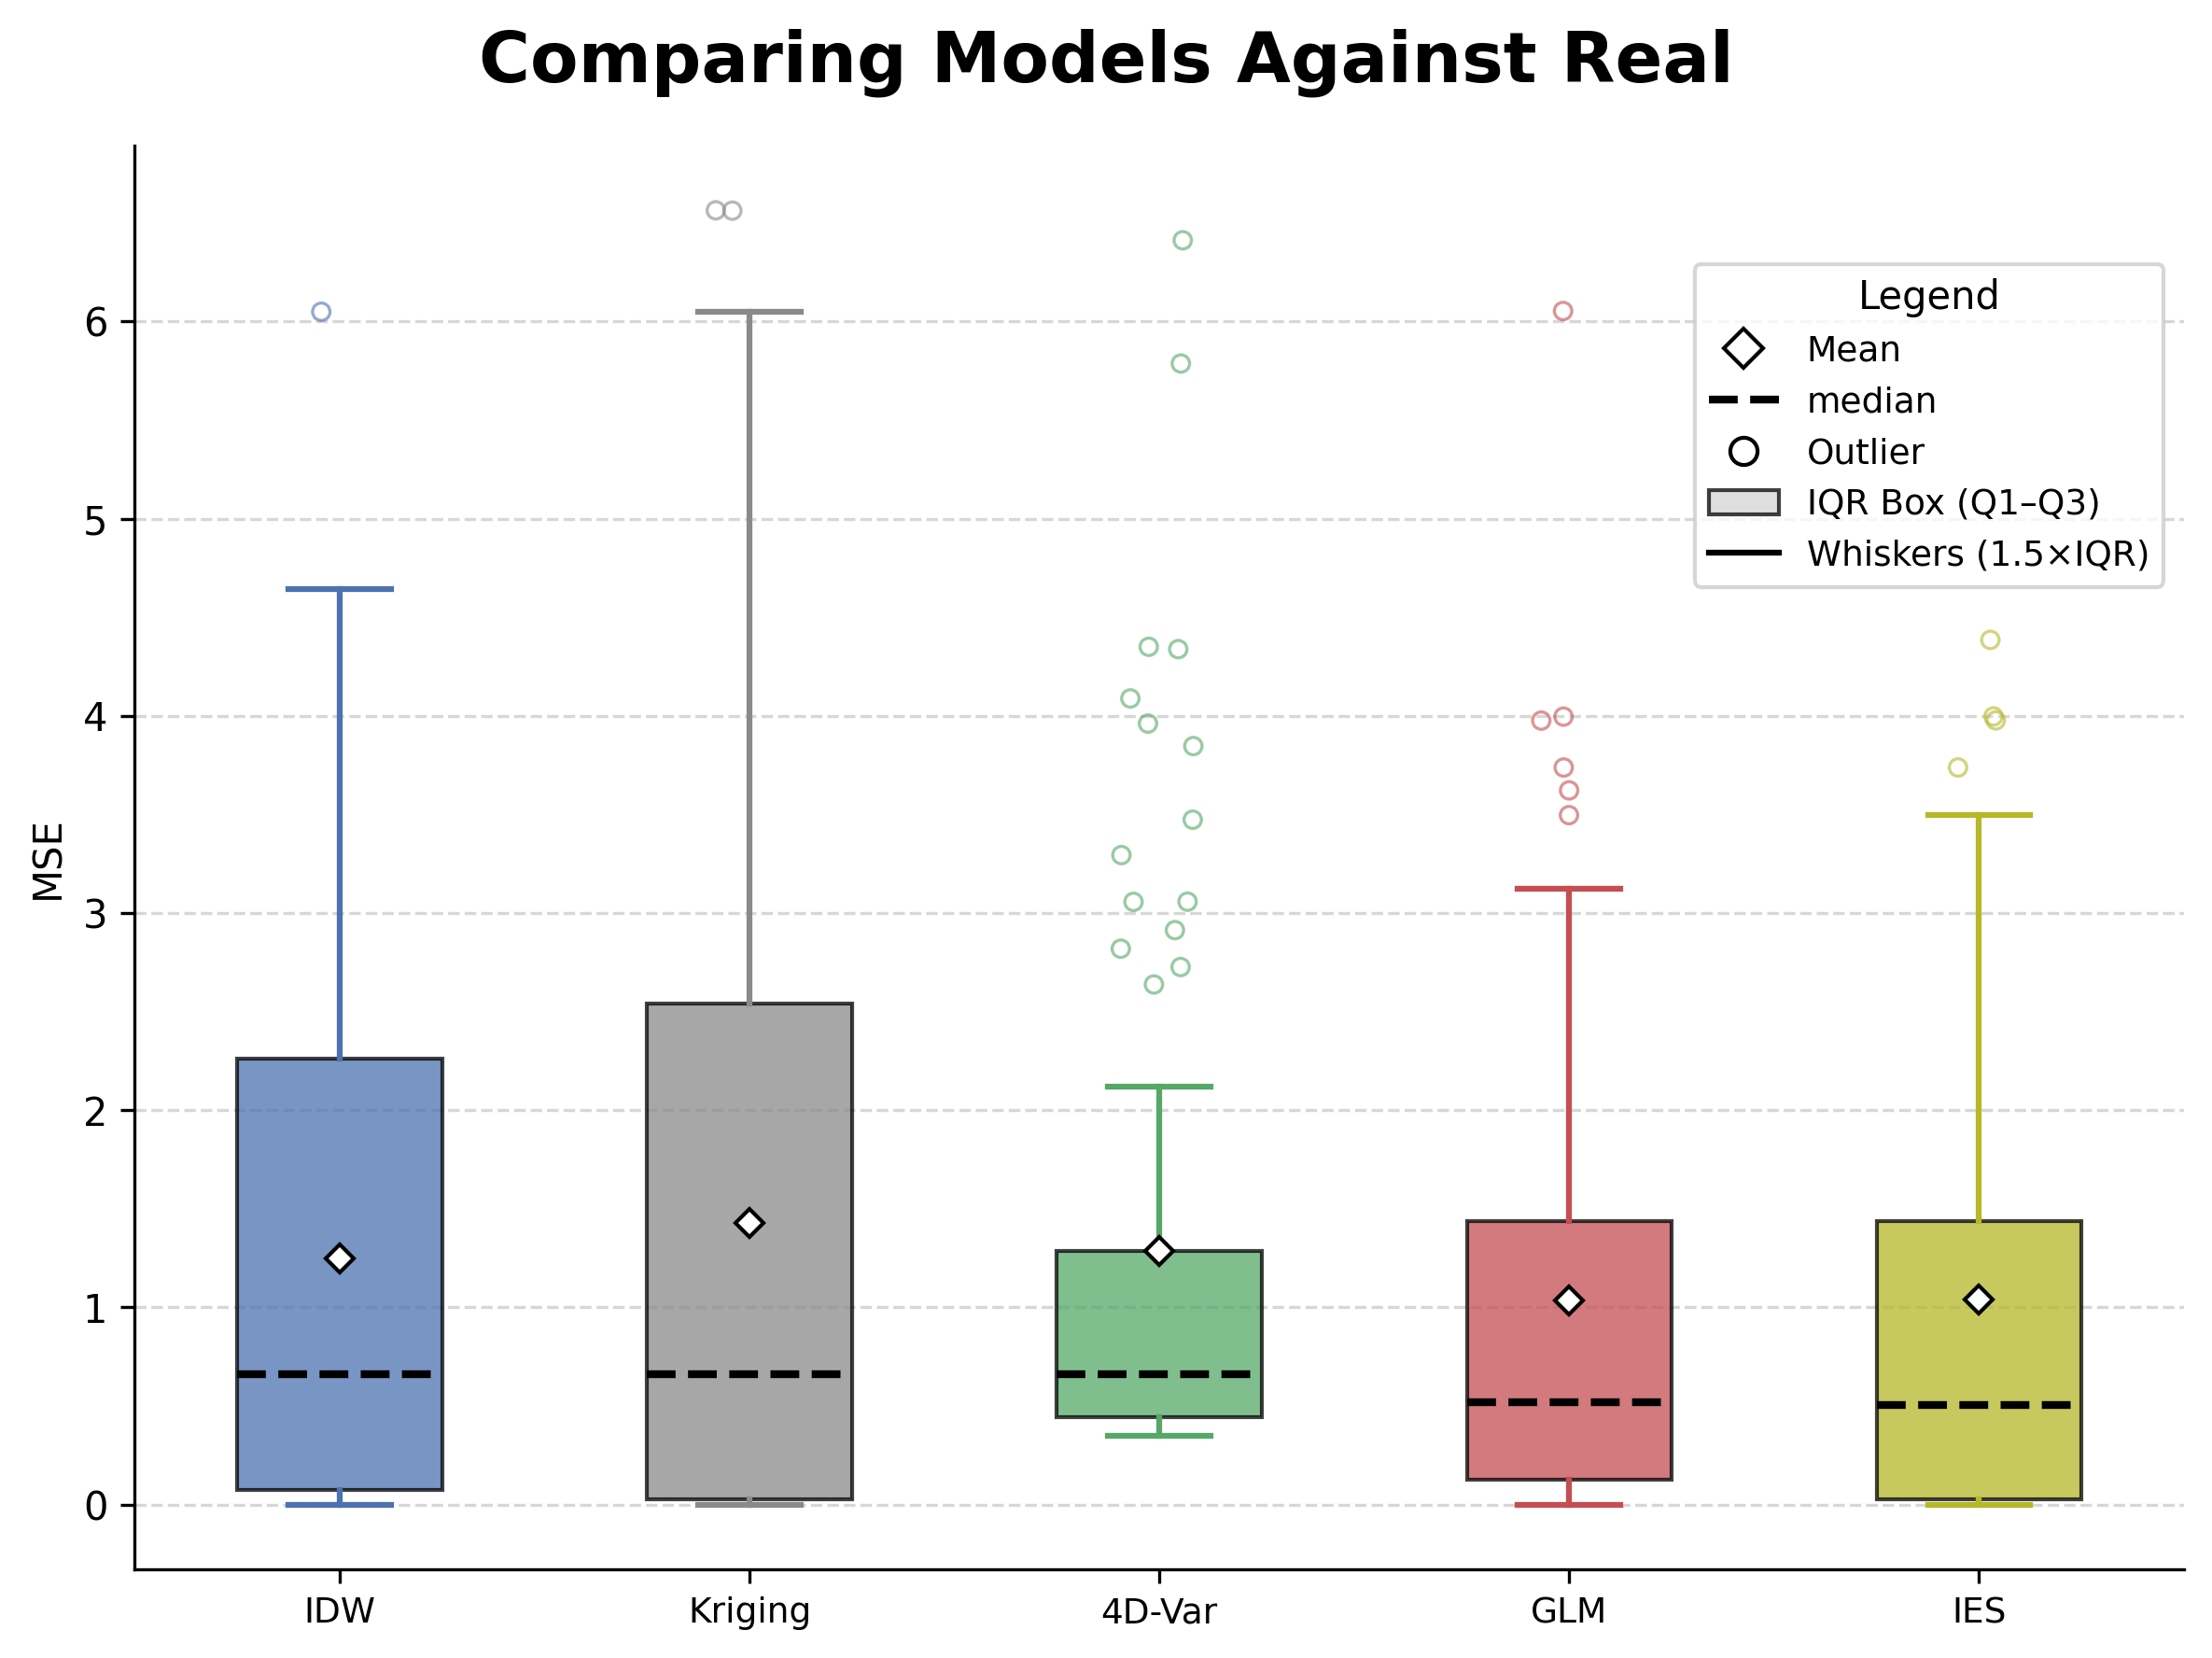
\includegraphics[height = 5in]{figures/boxplot_real.png}
\caption{Boxplot results for all $\realsize$ real-world samples evaluated by each method}
\label{fig:real_results_total}
\end{figure}

The real-world results are more compressed than the synthetic ones, reflecting the smaller absolute changes in PHC concentration observed in the field. Unlike the clear separation seen in the synthetic base case, the five methods now occupy substantially overlapping ranges, with median MSE values falling at 1.248 (IDW), 1.429 (Kriging), 1.287 (4D-Var), 0.1034 (GLM), and 1.038 (IES). GLM and IES retain a modest edge over the distance-based methods, with GLM achieving the lowest mean MSE and IES achieving the lowest median MSE overall, however the margins are close. 4D-Var no longer outperforms the distance-based methods on this dataset, recording both a higher mean and a higher median MSE than IDW, a reversal of the trend observed throughout the synthetic evaluation.

A key reason for this compression is that, unlike in the synthetic evaluation, the methods are supplied with measurements from only two of the three sensor locations at each stake, with the third held out for evaluation. This removes the truth concentrations closest to the boundary conditions supplied by the simulation, exactly where the parameter estimation methods showed their greatest advantage in the synthetic tests. Without that boundary information, the physics-informed optimisation provides less leverage, and IDW's simple spatial averaging becomes comparatively more competitive. The second reason for the compression is the smaller concentrations of PHC measured on average than the synthetic data represents. When all the measured concentrations of PHC are small, the pure distance-base metrics tend to perform better since they are unable to underestimate the unmeasured locations.

The decrease in performance of 4D-Var in particular is consistent with its performance under high soil parameter noise in the synthetic tests (Section~\ref{sec:res_measNoise}), where its comparatively simple gradient-based update was shown to be more susceptible to model mismatch than GLM or IES. Real soil is considerably more heterogeneous than the smooth, pilot-point-interpolated profiles used to generate the synthetic dataset, and 4D-Var's single-pass adjoint optimisation may converge to a poor solution when the true soil structure is substantially different from what the forward model can represent. GLM and IES, by contrast, incorporate iterative refinement and, in the case of IES, an ensemble of candidate solutions, which may make them more robust to this kind of structural mismatch. The wide, overlapping whiskers across all five methods further indicate that no single method reliably captures the individual variability of the 27 real-world samples, underscoring the difficulty of the field setting relative to the controlled synthetic conditions. Additional real-world samples, together with per-stake analysis of the specific soil conditions at each location, would help clarify whether this reversal reflects a general limitation of 4D-Var or is driven by a small number of poorly-suited stake locations.

% Auto-generated LaTeX table
\begin{table}[H]
  \centering
  \caption{Model performance on real-world data with sensor dropout (MSE)}
  \label{tab:sim_results}
  \begin{tabular}{lrrrrr}
  \toprule
  Condition & IDW & Kriging & 4D-Var & GLM & IES \\
  \midrule
  \multicolumn{6}{l}{\textit{Mean}} \\
  \hline
  Base Case & 1.248 & 1.429 & 1.287 & \textbf{1.034} & 1.038 \\
  10\% Sens Dropout & 1.259 & 1.483 & 1.293 & \textbf{1.032} & 1.083 \\
  50\% Sens Dropout & 1.243 & 2.192 & 1.272 & \textbf{1.015} & 1.094 \\
  50\% Sens Blackout & 1.248 & 1.554 & 1.265 & \textbf{1.024} & 1.025 \\
  \midrule
  \multicolumn{6}{l}{\textit{Median}} \\
  \hline
  Base Case & 0.6591 & 0.6591 & 0.6619 & 0.5198 & \textbf{0.5046} \\
  10\% Sens Dropout & 0.6591 & 0.6591 & 0.6408 & \textbf{0.4986} & 0.6917 \\
  50\% Sens Dropout & 0.6881 & 0.7812 & 0.6729 & \textbf{0.5633} & 0.8296 \\
  50\% Sens Blackout & 0.6591 & 0.6234 & 0.6244 & \textbf{0.501} & 0.5731 \\
  \midrule
  \multicolumn{6}{l}{\textit{Standard Deviation}} \\
  \hline
  Base Case & 1.411 & 1.731 & 1.346 & 1.245 & \textbf{1.174} \\
  10\% Sens Dropout & 1.412 & 1.824 & 1.349 & 1.248 & \textbf{1.124} \\
  50\% Sens Dropout & 1.361 & 3.369 & 1.277 & 1.23 & \textbf{1.106} \\
  50\% Sens Blackout & 1.411 & 2.27 & 1.315 & 1.244 & \textbf{1.118} \\
  \bottomrule
  \end{tabular}
\end{table}

To relate the real-world results back to the synthetic dataset, artificial sensor-dropout cases were also applied to the real-world data. These mirror the synthetic dropout conditions exactly: 10\% random measurement dropout, 50\% random measurement dropout, and a 50\% contiguous blackout in the middle of the simulation window, with aggregated results shown in Table~\ref{tab:sim_results} and visualized in Figure~\ref{fig:sim_sensDropout}. The trends are largely consistent with those recorded for the synthetic data in Section~\ref{sec:res_sensDropout}. The distance-based methods remain unaffected by the dropout, since they make limited use of the temporal measurements in the first place. Among the parameter estimation methods, performance improves slightly across all three dropout scenarios, most likely because the reduced temporal data limits overfitting and yields less aggressive estimates at unmeasured locations. However, given that the real-world dataset is considerably smaller than the synthetic dataset, this improvement may largely reflect sampling noise rather than a genuine effect.